% !TEX root = sirocco-main.tex

\section{Preliminaries}

In this section we fix our notation and prove some basic lemmas
required for the algorithm. We use standard notation from graph
theory and refer to the literature for extensive background. For an
undirected and simple graph~$G$ we denote by $V(G)$
the vertex set and by $E(G)$ the edge set of $G$. We also refer
to the literature, for the
formal definition of the LOCAL model of distributed computing.

A graph~$H$ is a minor of a graph~$G$, written~$H\minor G$, if
there is a set \mbox{$\{G_v :v\in V(H)\}$} of pairwise vertex disjoint and
connected subgraphs
$G_v\subseteq G$ such that if~$\{u,v\}\in E(H)$, then there is an edge
between a vertex of~$G_u$ and a vertex of~$G_v$. We call $V(G_v)$ the
\emph{branch set} of $v$ and say that it is
\emph{contracted} to the vertex~$v$.
%If $G_1,\ldots, G_k\subseteq V(G)$
%are pairwise vertex disjoint and connected subgraphs of $G$, then we write
%$G/G_1/\ldots/G_k$ for the minor obtained by contracting the subgraphs~$G_i$ (observe that the order of contraction does not matter as the
%$G_i$'s are vertex disjoint).

For a non-negative integer~$r$, a graph
$H$ is an \emph{$r$-shallow minor} of $G$, written
$H\minor_r G$, if there is a set~$\{G_v : v\in V(H)\}$ of pairwise
vertex disjoint connected subgraphs
$G_v\subseteq G$ of radius at most $r$ such that if~$\{u,v\}\in E(H)$,
then there is an edge between a vertex of~$G_u$ and a vertex of~$G_v$.
Observe that a $0$-shallow minor of $G$ is just a subgraph of $G$.

We write $\nabla_r(G)$ for $\max_{H\minor_r G}|E(H)|/|V(H)|$. Observe
that $\nabla_0(G)$ denotes the maximum average edge density of $G$
and $2\nabla_0(G)$ bounds the degeneracy of~$G$, which is defined
as $\max_{H\subseteq G}\delta(H)$. Here, $\delta(H)$ denotes
the minimum degree of~$H$.
%
A class~$\Cc$ of graphs has \emph{bounded expansion} if there is a function
$f:\N\rightarrow\N$ such that $\nabla_r(G)\leq f(r)$ for all graphs $G\in \Cc$.
This is equivalent to demanding that the degeneracy of each $r$-shallow minor
of $G$ is functionally bounded by~$r$.

We write~$K_{s,t}$ for the complete bipartite
graph with partitions of size~$s$ and~$t$, respectively. Observe that
$K_{t,t}$ has $2t$ vertices and $t^2$ edges, hence, if
\mbox{$\nabla_0(G)< t/2$}, then $G$ excludes $K_{t,t}$ as a subgraph.

For a graph $G$ and $v\in V(G)$ we write $N(v)=\{w~:~\{v,w\}\in E(G)\}$
for the \emph{open neighborhood} of $v$ and $N[v]=N(v)\cup\{v\}$ for
the \emph{closed neighborhood} of~$v$. For a set $A\subseteq V(G)$ let
$N[A]=\bigcup_{v\in A}N[v]$. We write $N_r[v]$ for the set
of vertices at distance at most $r$ from a vertex $v$.
A dominating set in a graph~$G$ is a set
$D\subseteq V(G)$ such that $N[D]=V(G)$. We write $\gamma(G)$ for
the size of a minimum dominating set of $G$. For $W\subseteq V(G)$
we say that a set $Z\subseteq V(G)$ \emph{dominates} or \emph{covers} or
is a \emph{cover} of $W$ if $W\subseteq N[Z]$.
Observe that we do not
require $Z\cap W=\emptyset$ as Czygrinow et al.\ do for covers.

\smallskip
The following lemma is one of the key lemmas used for the algorithm. It goes back to~\cite{lenzen2013distributed}.

\begin{lemma}\label{lem:neighborhood-dom1}
Let $G$ be a graph. Then there are less than $2\gamma(G)$ vertices $v$ with the property that $N(v)$ cannot be dominated by at most $2\nabla_1(G)$ vertices different from $v$.
\end{lemma}
\begin{proof}
Let $\gamma=\gamma(G)$ and $\nabla_1=\nabla_1(G)$ and assume that there are $2\gamma$ such vertices $a_1,\ldots,a_{2\gamma}$. We proceed towards a contradiction.
  Let $\{d_1,\ldots,d_\gamma\}$ be a minimum dominating set. At least $\gamma$ of the $a_i$'s are not in this dominating set. We can hence assume w.l.o.g.~that $\{a_1,\ldots,a_{\gamma}\}$ and $\{d_1,\ldots,d_\gamma\}$ are two disjoint sets of vertices.

We build a $1$-shallow minor $H$ of the graph $G$ with the following $2\gamma$ branch sets. For every $i\le \gamma$, we have a branch set
$A_i=\{a_i\}$ and a branch set $D_i=N[d_i]\setminus (\{a_1,\ldots, a_\gamma\}\cup \bigcup_{j<i}N[d_j] \cup \{d_{i+1},\ldots, d_\gamma\})$.
We call the associated vertices of $H$ $a_1',\ldots, a_\gamma',d_1',\ldots,
d_\gamma'$.

Since $\{d_1,\ldots, d_\gamma\}$ is a dominating set of $G$ and by assumption on $N(a_i)$, we have that in $H$, every $a'_i$ is connected to at least $2\nabla_1+1$ of the $d'_i$.
  We therefore have that $|V_H|=2\gamma$ and $|E_H| \ge \gamma(2\nabla_1+1)$, hence $|E_H|> |V_H|\nabla_1$, a~contradiction.
\end{proof}

Note that we cannot locally determine the number $\nabla_1(G)$.
We must hence assume that it is given with the input. Observe that
similarly, the algorithm of Czygrinow et al.\ works with the assumption
that the input excludes a complete graph with $t$ vertices as a topological
minor. This implies a bound on the edge density of topological minors
in $G$, which can be seen as being given with the input.

The algorithm proceeds in three phases. The first phase is
based on \cref{lem:neighborhood-dom1} as follows.
In the LOCAL model we can learn the distance-$2$
neighborhood~$N_2[v]$ of every vertex $v$ in $2$ rounds,
and then locally check
whether~$N(v)$ can be domi\-nated by at most $2\nabla_1(G)$
vertices.

\begin{tcolorbox}
% \fbox{
% \begin{minipage}{0.9\linewidth}
We let $D_1$ be the set of all vertices that do not have this
property. By \cref{lem:neighborhood-dom1}
we have $|D_1|\leq 2\gamma(G)$. We remove $D_1$ from the
graph and mark all its neighbors as dominated in one additional round.
% \end{minipage}
% }
\end{tcolorbox}


In the following we fix a graph $G$ and we assume that $N(v)$ can be
dominating by at most $2\nabla_1(G)$ vertices different from $v$
for all $v\in V(G)$. We write $\nabla_1$ for~$\nabla_1(G)$ and
we let $t\leq 2\nabla_0(G)+1$ be the smallest positive integer
 such that~$G$ excludes
$K_{t,t}$ as a subgraph. Note that this number is not required
as part of the input. We let $k\coloneq 2\nabla_1$.

\begin{example}
  A planar $n$-vertex graph has at most $3n-6$ edges. A minor of a
  planar graph is again planar, hence for planar graphs $G$ we have $\nabla_r(G) \leq 3$ for all $r\geq 0$ and $k=2\nabla_1(G)\leq 6$.
\end{example}

We also fix a minimum dominating set $D$ of $G$
of size~$\gamma$.
% In the following, when we speak of ``almost all vertices'', we mean all but at most~$c\gamma$ vertices for some
% constant $c$. This is again motivated by the argument that adding
% any~$c\gamma$ vertices
% to the dominating set will still give a constant factor approximation.
The following lemma is proved exactly as \cref{lem:neighborhood-dom1}.

\begin{lemma}\label{lem:neighborhood-dom2}
There are less than $2\gamma$ vertices $v$ with the property
that $N(v)$ cannot be dominated by at most $2\nabla_1$ vertices
from $D$ and different from $v$.
\end{lemma}

Unfortunately, we cannot determine these vertices locally, as it requires
know\-ledge of $D$, however, this structural property is very useful for
our further argumentation.

\begin{tcolorbox}
% \begin{minipage}{0.92\linewidth}
Denote by $\hat D$ the set of all vertices $v$
whose neighborhood cannot be dominated
by $2\nabla_1$ vertices of $D$ different from $v$.
Let $D'=D\cup \hat D$.
% \end{minipage}
\end{tcolorbox}

According to %\cref{lem:neighborhood-dom1} and
\cref{lem:neighborhood-dom2}, $D'$ contains at most
%$(1+4\nabla_1)\gamma$ vertices.
$3\gamma$ vertices.
% \alex{shouldn't we simply add $v$ in $D'$? We then get that $|D'|\le 3\gamma$.\\
%   $\gamma$ for $D$, and at most $2\gamma$ such vertices.}
Let us stress that~$D'$ will never be computed by our LOCAL algorithm. We only use
its existence in the correctness proofs.

\smallskip
We can apply these
lemmas to obtain a constant factor approximation for a dominating
set only if $\nabla_1(G)$ is bounded by a constant. For example in graphs of bounded degeneracy in general the number of vertices that dominate the
neighborhood of a vertex can only be bounded by $\gamma(G)$.
Hence, the approach based on covers and pseudo-covers that is employed
in the following cannot be extended to degenerate  graph classes.

\begin{example}
Let $G(\gamma,m)$ be the graph with vertices $v_i$ for $1\leq i\leq \gamma$,
$w^j$ for $1\leq j\leq m$ and $s_i^j$ for $1\leq i\leq \gamma, 1\leq j\leq m$.
We have the edges $\{v_1, w^j\}$ for $1\leq j\leq m$, hence $v_1$
dominates all $w^j$. We have the edges $\{w^j, s_i^j\}$ for all $1\leq i\leq \gamma,
1\leq j\leq m$, hence, the $s_i^j$ are neighbors of $w^j$. Finally,
we have the edges $\{v_i, s_i^j\}$, that is, $v_i$ dominates the $i$th
neighbor of $w_j$. Hence, for $m>\gamma$,
$G(\gamma, m)$ has a dominating set of size
$\gamma$ and $m$ vertices whose neighborhood can be dominated
only by $\gamma(G)$ vertices. \cref{lem:neighborhood-dom1} implies
that $\gamma < 2\nabla_1$, and as we can choose~$m$ arbitrary
large, we cannot usefully apply \cref{lem:neighborhood-dom1}.
Furthermore, $G(\gamma,m)$ is
\mbox{$2$-degenerate}, showing that these methods cannot be applied on
degenerate graph classes.

\begin{center}
  \begin{figure}
    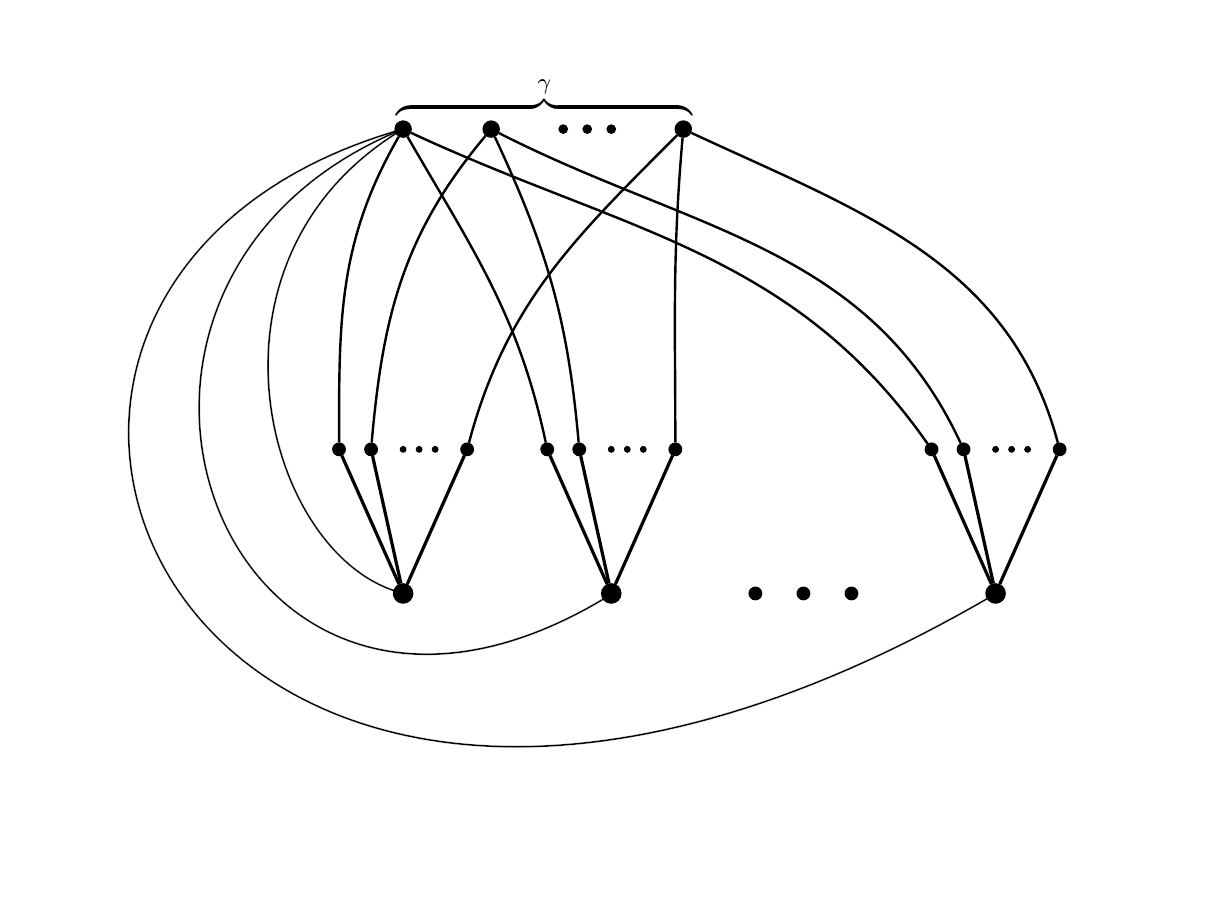
\includegraphics[scale=0.3]{ds1.png}
    \caption{ A $2$-degenerate graph where for many $v\in V(G)$ the set $N(v)$ can only be dominated by at least $\gamma$ vertices different from $v$. }
  \end{figure}
\end{center}
\end{example}
